\chapter{\deisa: \dask-Enabled In Situ Analytics}



\epigraph{\textit{If I have seen further, it is by standing on the shoulders of Giants.}} {Issac Newton}



\section{introduction}

\section{The Bridging Model between BSP and Distributed Task-Based Paradigms}\label{sec:btp}

\subsection{Motivation}\label{sec:btp:motivation}
As already mentioned in the previous chapters, the in situ paradigm is a brilliant alternative to the post hoc. However, it becomes quickly less relevant due to its setup complexity, as most of in situ tools are built on the MPI programming model which inherited from the host simulation. While MPI is one of the most relevant programming models for scientific application it is not suited for data analytics algorithms. To be able to explore the in situ paradigm with reduced complexity, we have mainly two possibilities: build both the simulation and the in situ tool with a higher-level programming model that makes the analytics easier to design; or keep the simulation built on MPI and propose a bridging model between MPI and another programming model which is more adapted for analytics.

The first possibility is not a relevant solution because it means that we will need to write simulation codes in another programming model, likely higher-level and slower, which is not a good idea for the reasons we mentioned in section\ref{BSP} about the success of MPI and BSP in general. 
The second possibility is more interesting as it will keep the BSP programming model for the simulations, choose a more adapted model for analytics and propose a bridging model to couple them. 
In this work, we have opted for the second solution and chosen the task-based programming model for the in situ analytics for the easiness it brings as well as the variety of tools that are already available and usable for different data processing. The following discussion only focuses on the BSP and the distributed task-based programming models, to showcase the challenges, however the proposed bridging model makes abstraction of the used models in both sides.  

The BSP and the Task-based paradigms differ not only in terms of abstraction levels, development effort, and performance but also in defining key concepts such as parallelism and the data and how they are managed.

First of all, the type of parallelism in BSP, let us take MPI as an example; the application is represented as a set of $P$ processes, each with its local memory and buffers. The parallelism in the task-based model is expressed in terms of tasks and dependencies. While the user is responsible for creating the processes and their management in MPI, a runtime ensures that job in task-based models. We talk about explicit parallelism in MPI and implicit one in the task-based programming model. 
Secondly, the data semantics and representation in those models are different too. As defined in MPI, the data are buffers that keep the same name during execution and whose values are updated as the simulation progresses. Hence the data in MPI can be defined as the value of a given variable at a specific moment.
In task-based models, data are immutable and defined either as an input or an output of a given task. While the timestep is important to identify needed data in MPI, it does not have a similar signification in a task-based model. 
The third big difference is related to the view we may have about an application in both cases. While a task graph describes all the tasks that will be run in a task-based model, it is complex and sometimes impossible for BSP applications to have such a view from the beginning. And this makes the coupling more challenging, as we do not have any a priori idea about what will be executed at runtime, the data that will be generated, and when they are shared.

Those conceptual differences make coupling codes coming from the two paradigms challenging. To reduce this complexity and take advantage of both paradigms, we propose the Bulk Task Parallel paradigm that brings together the BSP and the task-based paradigms. 


\subsection{The Bulk Task Parallel Bridging Model}\label{sec:btp:btpmdel}

We define the Bulk Task Parallel (BTP), a new bridging model that couples two parallel programming models. In the frame of this work, we only consider a producer/consumer scheme where the producer is parallelized following the BSP model and the consumer is in a task-based model.  The BTP is built on top of basic concepts, namely: BTP tasks (section~\ref{btptask}), exchange points (section~\ref{EP}) and delivery facilities (section~\ref{DF}).  

Let an \textbf{\textit{Actor}} be the union of a parallel code and all its necessary resources: processing and memory units.   
For instance, let $A_{BSP}^{R_{1}}$ be an \textit{Actor} where $A$ is a BSP implementation of a problem $P_{1}$, and $R1$ is the needed resources for $P_{1}$ to be run, and let $B_{Task}^{R_{2}}$ be an \textit{Actor} where $B$ is a Task-based implementation of a problem $P_{2}$, and $R_{2}$ is the needed resources.

The way an Actor is defined in BTP is different compared to the existing Actor models. An \textit{Actor} in BTP encapsulates a coherent parallel application, and supports communication with external ones. To our knowledge, that's the first model that proposes to loosely couple distributed applications this way. An \textit{Actor} in BTP is a more generalized concept, that can cover more use cases by supporting BTP tasks internally with no restriction on how the task works, or parallelized or not. In this work we show two different BTP actors implementations from two different programming models with different abstraction levels. The producer/consumer example for actors coming from two programming models is the smallest general coupling example that can be shown.

\subsubsection{BTP Tasks}\label{btptask}
Let $S_{BSP}^{R_{s}}$ be an iterative code (a simulation code for instance). Let \textbf{C} be a computation and let \textbf{Cmn} be a communication performed internally to the \textit{Actor} (MPI communication for instance). The smallest \textit{Task} that can be defined in a BSP model is the union of all computations \textbf{C} that are delimited by two communications \textbf{Cmn}. 

A \textit{BTP task} can be seen as a \textit{Task} where we distinguish internal and external communications. It is a set of computations \textbf{C} and internal communications \textbf{Cmn}, delimited by two \textit{Exchange Point} (a possible external communication). In \textit{Task-based} model we distinguish the internal (to the \textit{Actor}) input/output data from the external ones (where the source/destination) is another \textit{Actor}. Hence, a \textit{BTP task} is a subgraph that is delimited by two external communications done through \textit{Exchange Points}.


\begin{figure}[tb]\centering
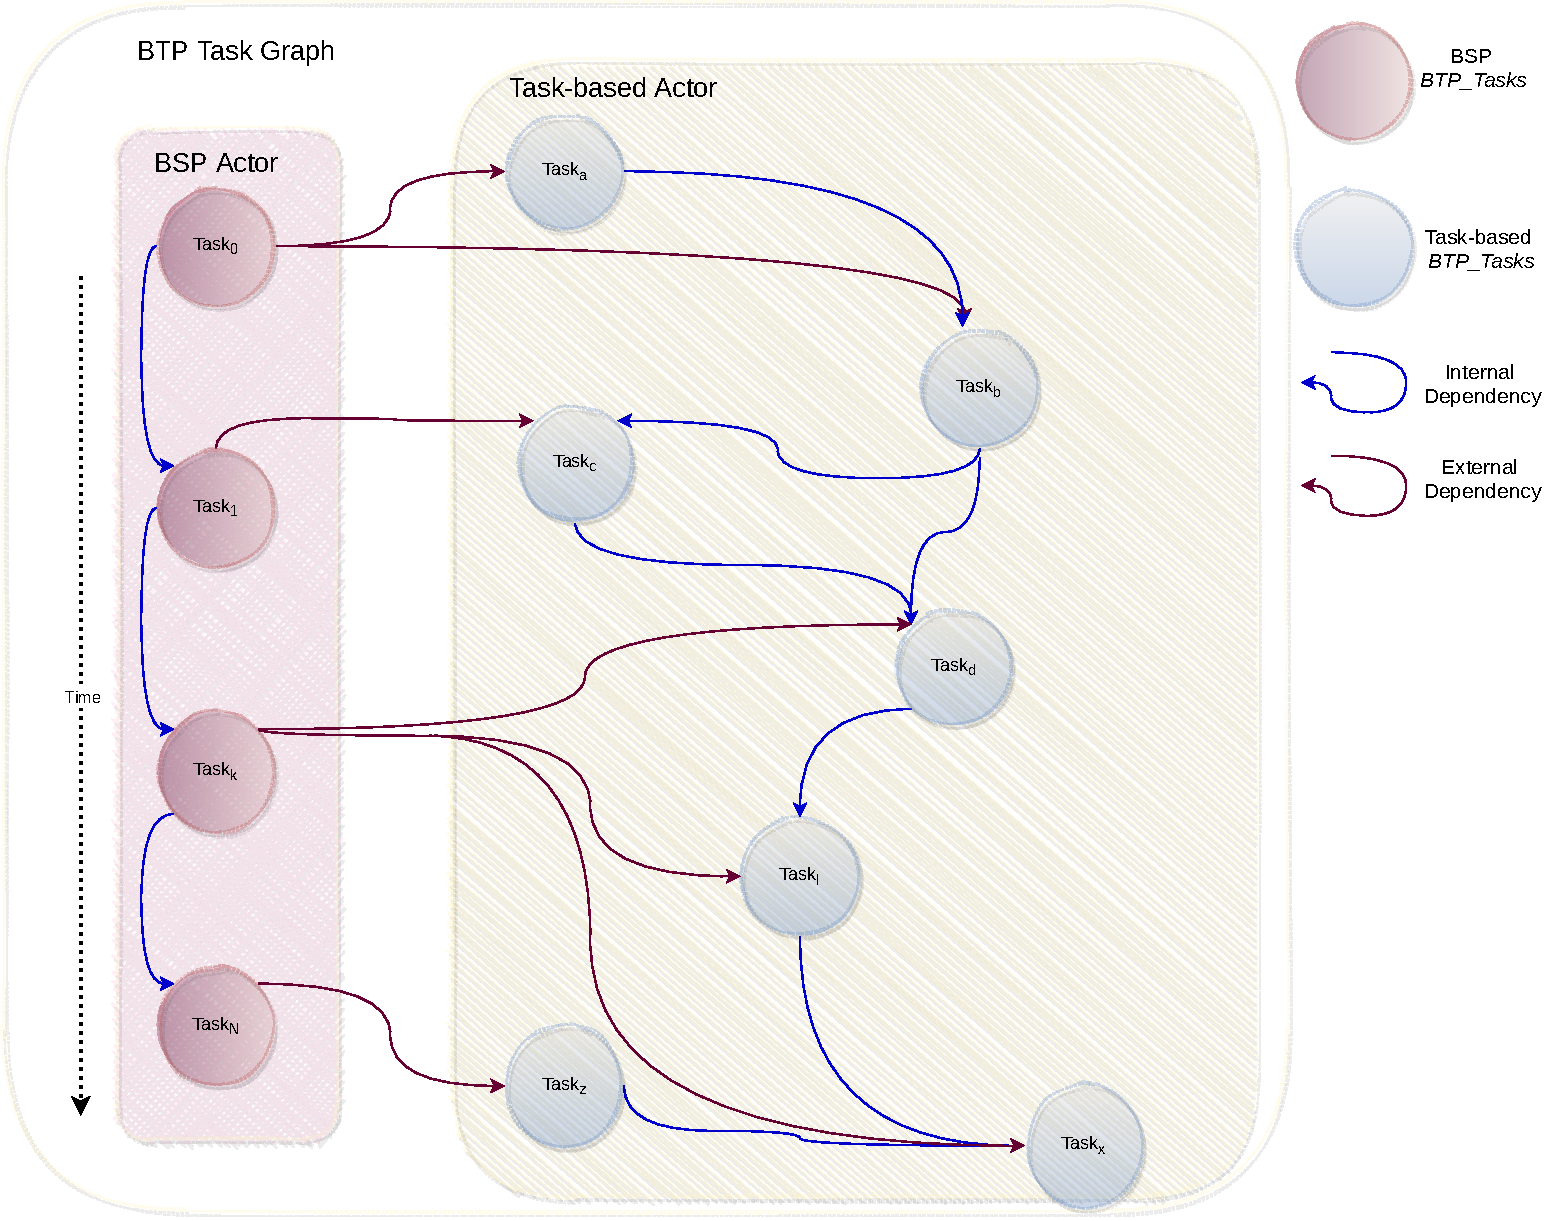
\includegraphics[width=0.75\columnwidth]{figures/BTPTaskGraph.pdf}
\caption{BTP task graph}
\label{figWUG}
\end{figure}

\subsubsection{Exchange Point}\label{EP}

An \textit{Exchange Point} (EP) can be defined as an entry point to BTP model. An \textit{Actor} shares through it an internal data with other \textit{Actors}. The main motivation to introduce \textit{Exchange points} is to keep a good separation of concerns. It provides a clean way to couple \textit{Actors}. For instance \textit{Actor A} can through its \textit{EPs} expose an array \textit{A} for external use. \textit{Actor B} does not need to know how \textit{Actor A} computes this array, and \textit{Actor A} needs to know neither which data \textit{Actor B} needs nor how it will use it.

The only way to get information about data an \textit{Actor} generates is by establishing a connection with it through a \textit{Delivery Facility} and checking available data (the data that \textit{A} wants to share) in the \textit{Exchange points}.


\subsubsection{Delivery Facility}\label{DF}

In addition of ensuring the establishment of connections between \textit{Actors}, the \textit{Delivery Facility} (DF) ensures a global identification and redistribution of data between \textit{Actors}. Hence,  it can be split to 3 main components : a \textit{Connection Facility} a \textit{Data Identification Component}, a \textit{Data Redistribution Component}.
\begin{itemize}
   \item \textit{Connection Facility} (CF): it establishes connections and communication with remote actors.
   
   \item \textit{Data Identification Component} (DIC): is responsible for the identification of a piece of data internally in an \textit{Actor} and translate its identifier to a global ID understandable in other \textit{Actors}. The step of identification is essential due to the different ways data is defined in the two paradigms. 
   
   \item \textit{Data Redistribution Component} (DRC): implements a data redistribution scheme. It is aware of the number of the resources $R$ (processes or workers) in the \textit{Actor} $Consumer_{Paradigm}^{R}$ and maps each data to a set of resources.
\end{itemize}

\subsection{Porting a BSP code to BTP semantic}\label{sec:btp:porting}

\begin{figure*}[tb]
\centerline{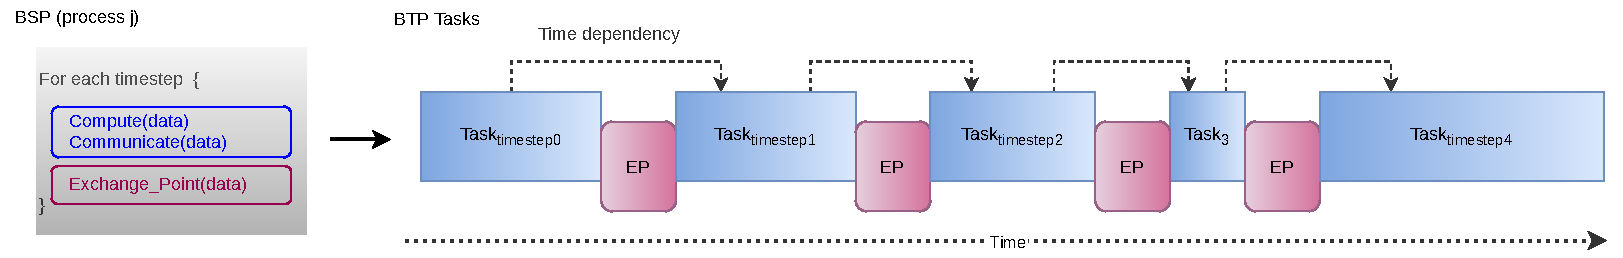
\includegraphics[width=\textwidth]{figures/unrolled.pdf}}
\caption{Example of BTP representation for an iterative BSP code}
\label{figunroll}
\end{figure*}

We suppose that the BSP \textit{Actor} is an iterative code parallelized in MPI. The code does not need to be rewritten to be designed in the BTP semantic. What needs to be done is only to tag the data we want to share externally and specify when this will be done. Concretely, calls to \texttt{Exchange\_point} are added in the simulation code to make data available for external use. By definition, a \textit{BTP task}, in BSP words, is a set of computations and internal communications that are delimited by two \textit{EPs}; concretely, it is all the code that is delimited by two calls of \texttt{Exchange\_point}. The call to \texttt{Exchange\_point} that is added at the end of each iteration in the loop in fig.~\ref{figunroll} is enough to construct a list of \textit{BTP tasks}, one per each time step. It is similar to an unrolled loop over time.


\subsection{Full Producer Consumer Example}\label{sec:btp:FullPCExample}

 
\begin{figure}[tb]\centering
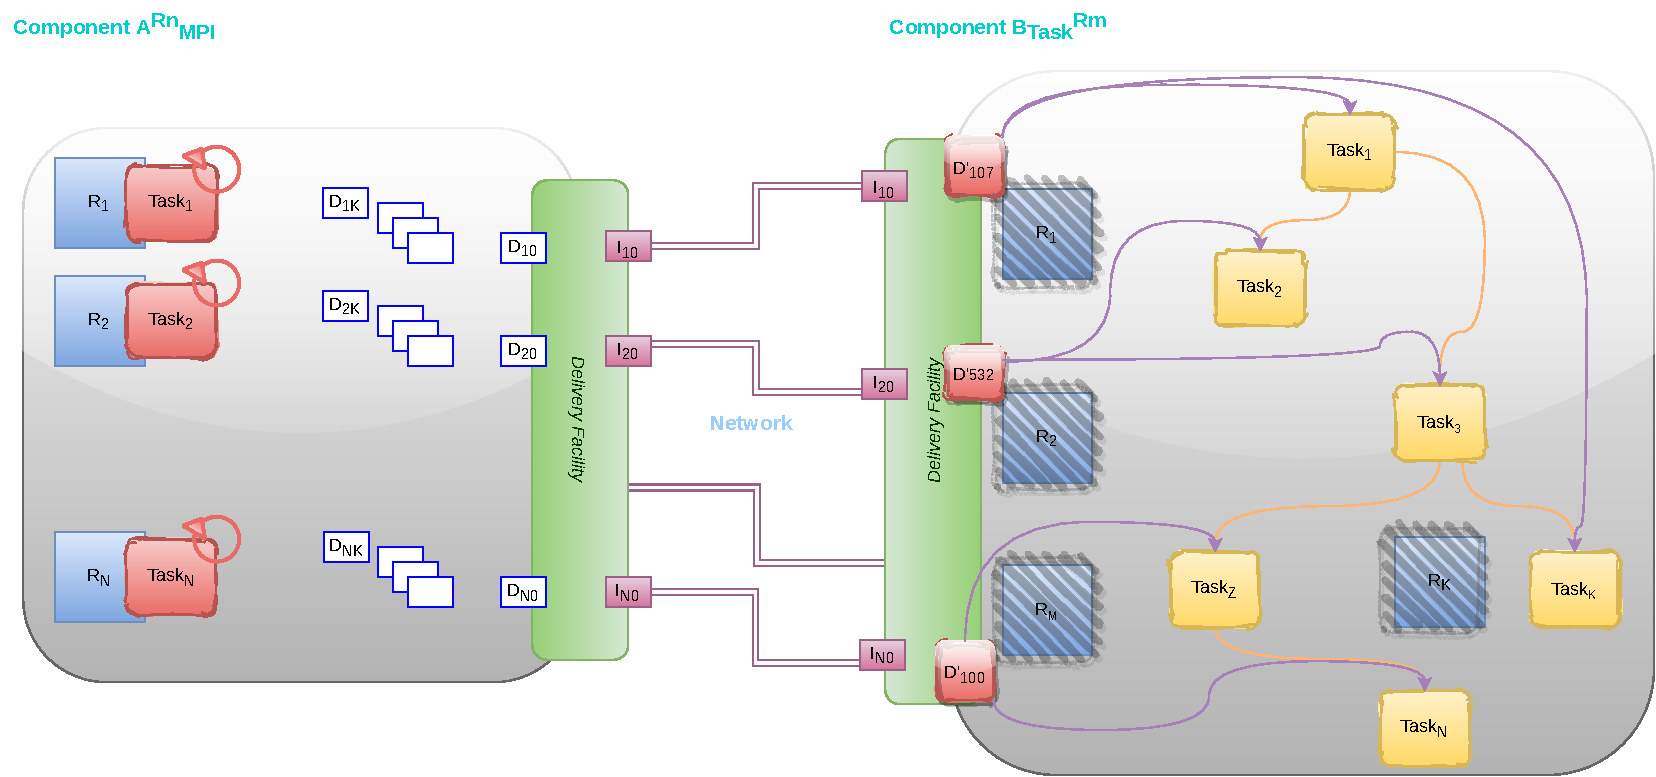
\includegraphics[width=\columnwidth]{figures/BTP.pdf}
\caption{producer consumer example}
\label{figBTP}
\end{figure}

Figure~\ref{figBTP} shows an example coupling $A_{BSP}^{R_{n}}$ and $B_{Task}^{R_{m}}$ where \textit{Actor A} is a producer and \textit{Actor B} is a consumer. The BSP \textit{Actor} has $R_{n}$ resources. Each $Task_k$ is scheduled explicitly to a set of resources $R_{k}$. In scientific applications, we usually have an iterative code. Each \textit{Task} generates a block of data at a given timestep $t$ (only one \textit{Task} is shown in the figure, with a loop mark). Those blocks of the data (small blue boxes $D_{i,j}$) are shared through the \textit{Exchange points} (not represented in the figure) and sent to the \textit{Delivery Facility}.
\textit{Actor B} is the consumer of the data. It is a task-based \textit{Actor}, has $R_{m}$ resources that are managed implicitly by a runtime (blue boxes with grey hachures). A task graph is represented as a BTP \textit{Task} graph (yellow graph), with dependencies on external inputs. Those inputs (in red) are data with new keys (IDs) that are easily recognizable, thus usable in \textit{Actor B}.  

The data are sent through the network between \textit{Actors}. The \textit{DFs} ensure the connection to a distant \textit{Actor}, the identification and redistribution of data between \textit{Actors}. 
In this figure, the data identification is made in two steps from each side. The small blue boxes $D_{i,j}$ are identified by three elements: $D$ is the name of the data, $i$ is the MPI rank (for instance or the position of this block of data in the global distribution), and the $j$ corresponds to the timestep. These keys can be considered as local to the \textit{Actor A}. 
In the same Actor, a new key has been created $I_{l,m}$. It is a global key recognizable in the \textit{DF} of \textit{Actor B}. In the \textit{Actor B}, those keys are translated to new keys internally understandable $D'_{k}$. 
This identification and translation process can be done in fewer steps. For example, if $I_{l,m}$ is recognizable by \textit{Actor B}, then there is no need for further translation at reception.

\section{BTP Implementation}\label{sec:btpimplementation}
Several choices have been made regarding the implementation of the BTP paradigm. We have focused on three main goals: performance and separation of concerns on the simulation side and productivity on the analytics side. All our choices have been guided by those goals to propose a solution that responds the most to the main motivation of this thesis, namely: bringing together the performance of in situ and the productivity we were used to in post hoc workflows, for that we have opted to use focus on the MPI implementation of BSP to parallelize simulation codes, \pdi data interface to handle data and implement the \textit{Delivery facily} engine, \dask distributed as a task-based framework to introduce a distributed pythonic environment in in situ paradigm. 
We have chosen MPI for its success and popularity in the HPC community; all legacy and new production codes are parallelized in MPI+X. We will focus here on justifying our choice regarding \pdi and \dask.

As already presented in section~\ref{sec:pdi}, \pdi is a lightweight data handling library that keeps an outstanding separation of concerns. With its declarative API, it enables sharing of simulation data for external use without any copy, thus its performance. In addition, it allows changing the data handling approach in the external configuration file without recompiling the simulation code. \pdi is already used in several production codes such as Gysela\cite{bigot:hal-01050322-gysela, latu:hal-01834323-gysela, latu:hal-01719208-gysela} to handle their IOs with \texttt{decl'hdf5} or for check-pointing using \texttt{FTI} plugin.      
In this work, we have chosen to use \pdi to extract simulation data as an \textit{Exchange Point}, and implemented the \textit{Data Facility} through a new \pdi plugin named \deisa. In addition to the advantages listed above, \pdi allows switching between different plugins easily, thus switching between in situ and post hoc modes; such an advantage is crucial to support heterogeneous workflows to be able to keep analytics results along with brute data in case further analytics are needed. 

One of the main issues in the in situ approach is its setup complexity. In this work, we introduce an outstanding ease-of-use in in situ workflows which is comparable to post hoc ones and bring the zen of python to the HPC community, all in one through \dask distributed. Among other data analytics frameworks, we have opted for \dask (to be our distributed task-based framework) because it offers distributed APIs for well-known python libraries such as \texttt{numpy}, \texttt{pandas} and \texttt{scikit-learn}. A post hoc sequential python code is easily ported to in situ distributed \dask code thanks to BTP paradigm.     


\subsection{Data Model}\label{sec:btpImp:datamodel}
Data is one of the core concepts of our work; its definition, identification, representation, and communication are as important as its processing. To smooth  differences between BSP and task-based model(mentioned in section~\ref{sec:btp:motivation}), the \textit{Delivery Facilities} from both sides, being aware of the semantics of data, add a layer to make it understandable in the other model. We will detail in the following sections how we managed the data in BTP regardless of all the differences in data semantics and definitions.

\subsubsection{Data Semantics}\label{sec:datamodel:datasemantic}

In this section, we will recall the difference between the semantics of data in the two models; this is important because all the following sections are based on those definitions.

\paragraph{Definition:}\label{defdataBSP}
In the BSP model, data can be defined as a value of a buffer at a given timestep. In MPI, the name of this buffer, an MPI communicator, the rank of the process, and the timestep are needed to identify a data in the global distribution of the array generated by a simulation over time. 

\paragraph{Definition:}\label{defdatataskbased}
Data in task-based model is an immutable object and can be defined as an input and/or an output of a given task. In \dask a data can be seen as a specific task called \textit{pure data task} (see section~\ref{sec:puredata}). It is identified by a unique \textit{key} in \dask task-graph. 

In order to couple a BSP \textit{Actor} and a task-based one, we have to map data generated by the first to the task-graph managed by the second.
A possible way to do that is to this is by uniquely identifying the data generated by the simulation (as defined in \ref{defdataBSP}) and mapping it as an input to the task graph as a \textit{pure data task}. Such a mapping keeps the properties of each model and does not -violate- the definitions of data in both models.


\subsubsection{Data Definition}\label{sec:datamodel:datadef}
%from ptr - pdi store -  pybind - numpy - dask
% configuration file
\begin{lstlisting}[float, label=ymldata, language=yaml, caption=Data description in \pdi \deisa YAML file]
pdi:
    types: #[...] including config_t description
    metadata: {step: int, cfg: config_t, rank: int} |\label{ymldata:metadata}|
    data: |\label{ymldata:data}|
        temp: # the main temperature field |\label{ymldata:temp}|
            type: array |\label{ymldata:temp.type}|
            subtype: double |\label{ymldata:temp.subtype}|
            size: [ '$cfg.loc[0]', '$cfg.loc[1]' ]  |\label{ymldata:temp.size}|
    plugins:
        mpi: # get MPI rand and size
        deisa:
            scheduler_info: scheduler.json
            init_on: init 
            time_step: $step 
            deisa_arrays: # Deisa Virtual arrays
                G_temp: # Field name
                    type: array
                    subtype: double
                    size:
                        -'$cfg.maxTimeStep'
                        -'$cfg.loc[0] * ($rank % $cfg.proc[0])'
                        -'$cfg.loc[1] * ($rank / $cfg.proc[0])'
                    subsize: [1, '$cfg.loc[0]', '$cfg.loc[1]'] # chunk size
                    start:  # chunk start
                        -$step
                        -'$cfg.loc[0] * ($rank % $cfg.proc[0])'
                        -'$cfg.loc[1] * ($rank / $cfg.proc[0])'
                    +timedim: 0 # a tag for the time dimension
            map_in: # deisa array mapping
                temp: G_temp    
\end{lstlisting}


\pdi is process-local. When data is shared with \pdi, it only gets a pointer to that data rather than making a copy unless it is defined as metadata in the specification tree (see section~\ref{sec:pdi} for more details about \pdi). 
\deisa plugin is built on \pdi with python support, and \pdi uses already \texttt{pybind11} to expose C++ types to python, thus \deisa uses it too. 
When data is shared with \pdi and has to be handled by \deisa, a pointer of that data is passed to \pdi and transformed into a \texttt{numpy} array by \texttt{pybind11} then passed to the \deisa plugin. 
The plugin calls \pydeisa library, which is a python library that implements the \textit{DF} concretely.
Note that there is no copy that is performed, and all those steps are done in the master thread of the MPI process sharing its data. 

The data definition for the simulation \textit{Actor} ends here. We will detail the communication in section~\ref{sec:DandCcomm:data}.

In \dask side, we create a \texttt{dask.array} from a set of metadata; we have implemented two solutions, a synchronous one, where a \texttt{dask.array} is created per timestep once the simulation data is sent to the workers and an asynchronous version where a \texttt{dask.array} is created even before the simulation starts generating the array. 


\subsubsection{Data Representation}\label{sec:datamodel:datarepresent}

%Deisa virtual arrays in synch or numpy arrays in asynch and dask arrays 
%from the simulation side as a mirror of the dask array that we create in the client side.
In \dask our data is represented as \texttt{dask.array}s. This representation has the advantage of keeping decomposition information of out-of-memory problems, through chunks definition. A similar representation has been used in several tools. A \textit{dask.array} is similar to an HDF5 and PycompsS datadets. 
We have added a support for a similar representation of data in \deisa plugin, called \deisa virtual arrays. We have two main motivations behind that: the first point is having a way to describe the spatio-temporal decomposition, and the way each block of data generated by a local process is mapped to the global array; the second one is to gather all needed metadata (regarding types, sizes, subsizes) and send them at once to minimize the load in the scheduler.   
We suppose that we have a perfect decomposition in the simulation side, that is all processes have the same size of data. 

We have added three main sections in the \deisa plugin configuration file:
\begin{itemize}
    \item a \texttt{deisa\_virtual\_arrays} section that describes the global data arrays following time and space distributions, independently from local data name,
    \item a \texttt{map\_in} section that maps local buffer's name (defined in the \texttt{data} section of \pdi) to the \texttt{deisa\_virtual\_arrays}'s name,
    \item an \texttt{init\_on} initialization event to gather all the needed metadata data and send them to the \textit{DF} of \dask \textit{Actor}. The needed metadata have to be shared by the simulation before the \texttt{init\_on} event is issued. 
\end{itemize}

%(discussion sur les differentes facons de represneter les donnees dist)
%Dask Arrays Pycomps datasets Legion smartsim dataspaces

\subsubsection{Data Identification}\label{sec:datamodel:dataid}
%metadata
%what and how and why 
%keys we get from a scatter, the size and position are sent 
%used for dask array creation 

To smooth the differences in the data semantics, we uniquely identify each value of a given buffer produced in the BSP model. This step is made in the \textit{Data Identification Component}; it consists of associating a unique \textit{key} to a buffer's value at a given timestep, and using this same \textit{key} in the creation of the corresponding \texttt{dask.array}.

\paragraph{Synchronous Implementation}
In the synchronous implementation, our solution is based on \dask \textit{key} management system with a set of metadata. Once data is generated by an MPI process, a set of metadata is associated with it. The metadata contains the name of the buffer, the position of the data in the global domain decomposition and the current timestep. The \textit{key} of the \texttt{Future} returned by the \texttt{scatter} function that we have used to send the arrays from the MPI processes to \dask workers is appended to the metadata and sent to the scheduler. The \textit{key} returned by the \texttt{scatter} is unique. Thus the data (a value of a buffer generated by a process at a given timestep) can be identified in \dask as an immutable object, identified by that unique \textit{key}. 

\amal{create an array for future example} 

\paragraph{Asynchronous Implementation}
In the asynchronous implementation of our system, the analytics task graph is submitted at the very beginning of the simulation. This becomes possible to three new concepts that we have introduced: 
\begin{itemize}
    \item \deisa virtual arrays (see section \ref{sec:datamodel:datarepresent}), that allow gathering needed metadata for \textit{dask.array}s creation. 
    \item contracts that have been introduced in\cite{mommessin_automatic_2017}. they allow extracting at the producer only needed data for analytics. 
    \item \texttt{external} tasks that make \dask distributed support unknown external data to be integrated into a task graph. 
\end{itemize}

Unlike the synchronous version where the \texttt{dask.array}s are built on chunks whose \textit{keys} are generated by \dask itself (that are returned by the \texttt{scatter}). In this version, we have created and used specific \textit{keys} to identify our data while keeping their semantics. Each \textit{key} contains 3 main sections:  the prefix \textit{external}; the name of the data and the position of the chunk is the global array considering both time and space decomposition. For example in  \texttt{(external-temp,(1,3,5))}, \texttt{temp} is the name of the data, $(1,3,5)$ is its position in the global array. This naming scheme can be extended to support multiple simulations as producers of data, feeding the same \dask cluster, by adding an identifier for the simulation, for instance. Those \textit{keys} are created when the corresponding data is available and is included in the contract (needed by the analytics).  

%%%%%
At the beginning of the simulation, the \textit{DF} connects to \dask, and sends the \deisa virtual arrays description to the \textit{DF} of \dask. The analytics client in \dask, makes selections using \texttt{slice} objects in the \deisa arrays depending on the pieces needed for analytics. Then send back the selections to the simulation \textit{DF}.

The contracts in the simulation side are checked every time data is available in a process; if this block is included in the selection needed by the analytics, then the associated \textit{key} is created, and the data (identified by this created \textit{key}) is sent to a pre-selected worker. In the \dask side, the contracts are used at the beginning to create the corresponding \textit{dask.array}s to the \deisa virtual arrays. similarly, \textit{keys} are created the same way in the \textit{DF} of \dask. Those \textit{keys} are used to identify the chunks of the \texttt{dask.array} associated with that data. This way, only the description of the arrays sent in the contract process is performed; no need to send more metadata at each timestep.  

\amal{example}

\subsection{Data and Control Communication}\label{sec:DandCcomm}
%possible push/pull, we opted for push


\subsubsection{Control Communication}\label{sec:DandCcomm:control}
All control goes through the scheduler, but we can optimize it through mpi as future work 
\paragraph{Queues} 

\paragraph{Variables}
when several clients need the same data 

\subsubsection{Data Communication}\label{sec:DandCcomm:data}
\paragraph{Deisa Bridge}
deisa plugin/ pycall
light client + far heartbeat 
limit 512 ..




\subsection{Data Flow}
limit generated data, but steering in the other sense can be done easily  
\subsubsection{Queues}
\subsubsection{Contracts}

\subsection{Dynamic scheduling}
\amal{triggers I have to do that }






\subsection{\deisa prototype}
\cite{deisa}

\subsubsection{Architecture}
\begin{figure}[tb]\centering
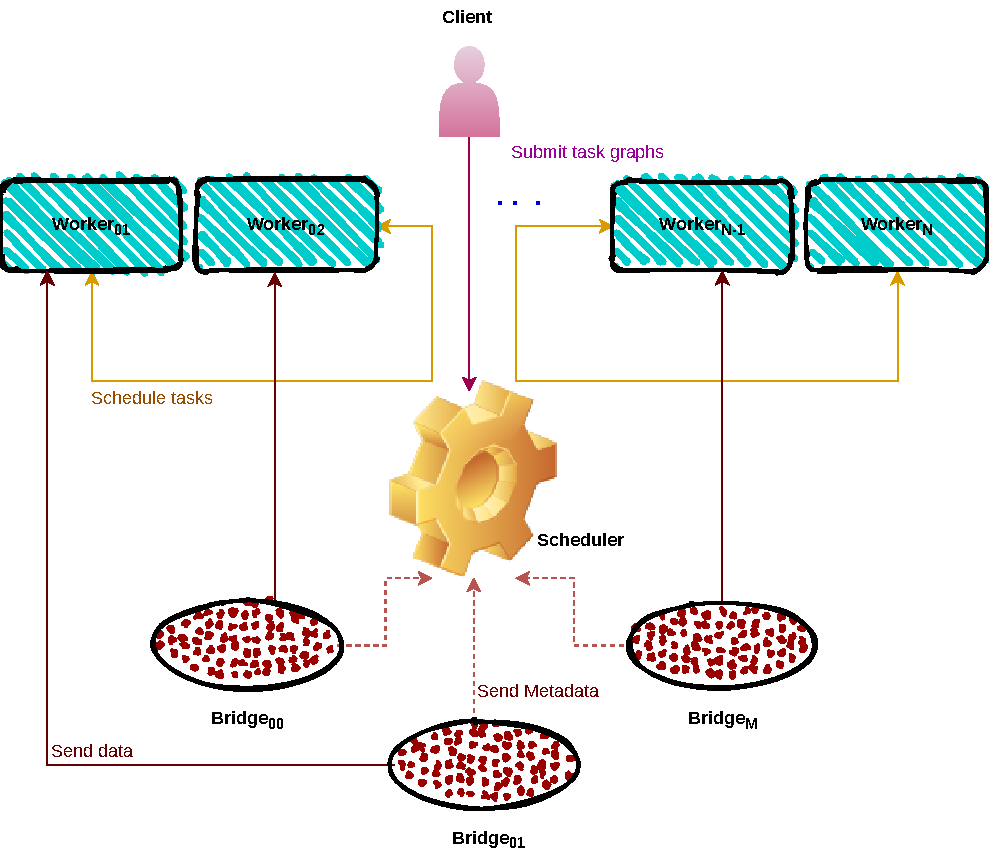
\includegraphics{figures/ArchiectureDeisa.pdf}
\caption{\deisa}
\label{figdeida}
\end{figure}


\subsubsection{API}
just the last one 
\subsubsection{Instrumentation}

\subsubsection{Evaluation}
\subsubsection{Limitations}
\section{\deetita: \dask-Enabled External Tasks for In Transit Analytics}

\begin{figure}[tb]\centering
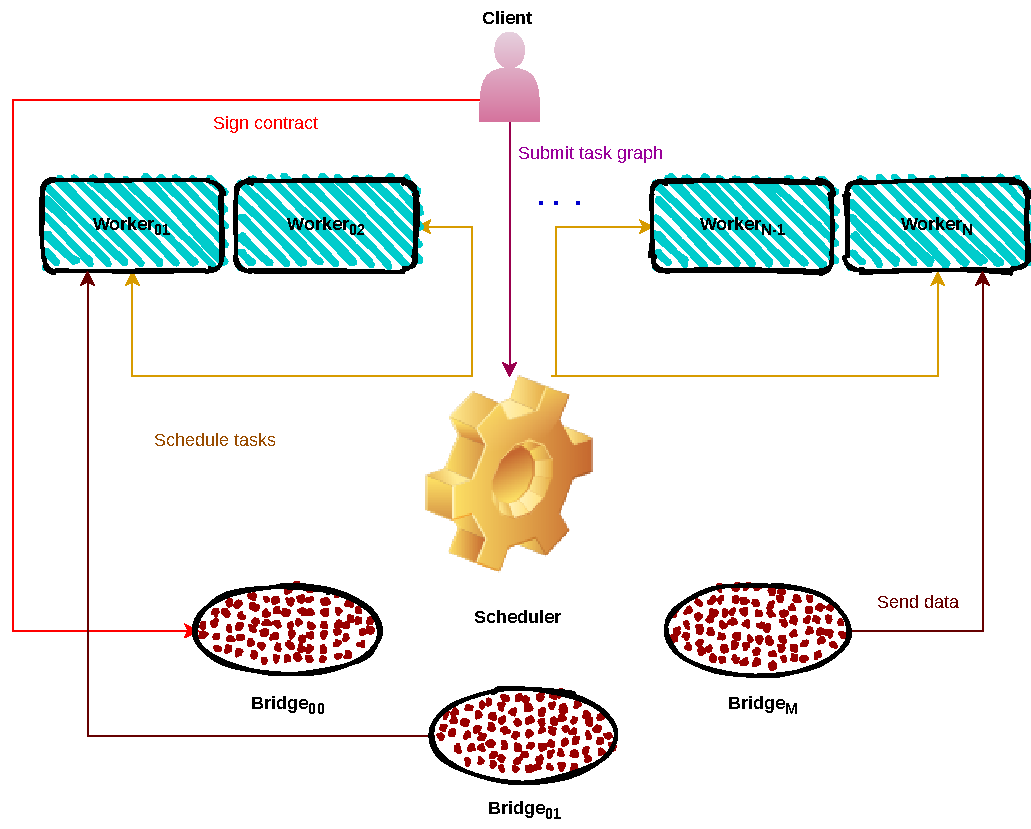
\includegraphics{figures/ArchiectureDeisaV2.pdf}
\caption{\deisa v2}
\label{figdeidav2}
\end{figure}
\subsection{\dask distributed external tasks}
\subsection{Asynchronous scheduling}
\section{Conclusion}